\documentclass{article}
\usepackage{amsmath}
\usepackage{graphicx}
\usepackage{tabularx}
\usepackage{array}
\graphicspath{ {./images/} }
\usepackage{geometry}
\title{Assignment 3 Report}
\author{Leonardo Celi \& Oways Jaffer \\ lgc59-omj9}
\date{}

\begin{document}

\maketitle

\section*{Project details}

\noindent \textbf{Language:} Python \\
\textbf{Libraries used:}  numpy, matplotlib.pyplot, functools, argparse, gtsam, scipy.optimize, networkx, matplotlib.animation.
\section*{Testing and Visualizations}
\subsection*{1 Potential Function (Testing Report)}
\subsubsection{Trial 1}

\begin{itemize}
    \item \textbf{Environment:}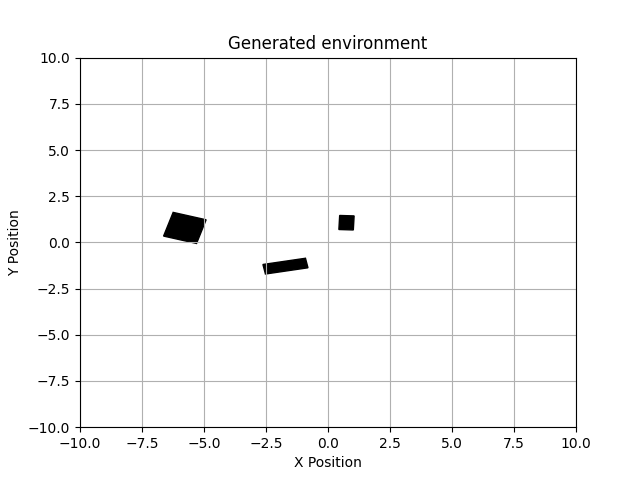
\includegraphics[scale=0.5]{asss3/images/pot1.png}
    \item \textbf{Number of obstacles}: 3
    \item \textbf{Start/goal configurations}: 
    \begin{enumerate}
        \item (0.0, 0.0) → (-5.0, 6.0)
        \item (4.0, 6.0) → (-7.0, -8.0)
        \item (-2.5, 4.0) → (-9.0, 6.0)
        \item (-1.0, 8.5) → (3.0, -4.0)
        \item (-8.0, 8.5) → (8.5, -8.0)
    \end{enumerate}
    \item \textbf{Success rate}: 100\% (5/5)
    \item \textbf{Average duration of path search}: 0.003841 seconds
\end{itemize}

\subsubsection{Trial 2}

\begin{itemize}
    \item \textbf{Environment:}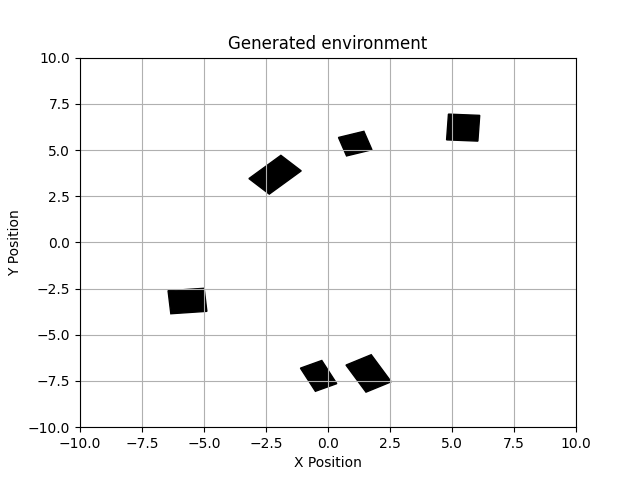
\includegraphics[scale=0.5]{asss3/images/pot2.png}
    \item \textbf{Number of obstacles}: 6
    \item \textbf{Start/goal configurations}: 
    \begin{enumerate}
        \item (0.0, 0.0) → (-5.0, 6.0)
        \item (4.0, 6.0) → (-7.0, -8.0)
        \item (-7.5, 4.0) → (5.0, -3.0)
        \item (-1.0, 8.5) → (3.0, -4.0)
        \item (0.0, 8.5) → (8.5, -8.0)
    \end{enumerate}
    \item \textbf{Success rate}: 80\% (4/5) 
\textit{Failure}: For configuration 2, the algorithm couldn't find a collision-free path as all recognized paths were collision-prone.

    \item \textbf{Average duration of path search}: 0.007825 seconds
\end{itemize}

\subsubsection{Trial 3}

\begin{itemize}
    \item \textbf{Environment:}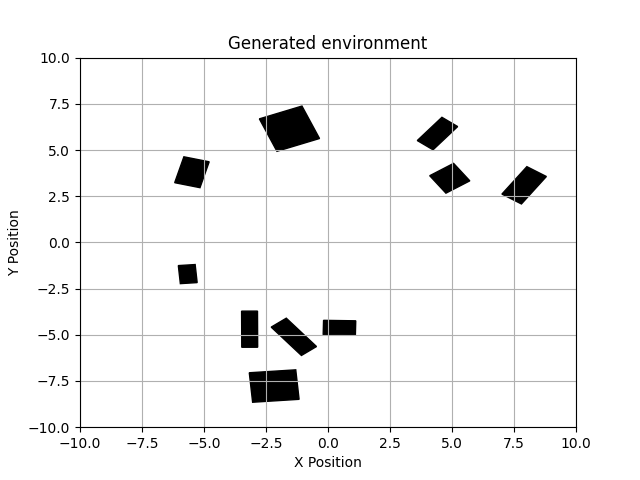
\includegraphics[scale=0.5]{asss3/images/pot3.png}
    \item \textbf{Number of obstacles}: 10
    \item \textbf{Start/goal configurations}: 
    \begin{enumerate}
        \item (0.0, 0.0) → (-5.0, 6.0)
        \item (4.0, 6.0) → (-7.0, -8.0)
        \item (-7.5, 4.0) → (-5.0, -8.0)
        \item (-1.0, 8.5) → (3.0, -4.0)
        \item (0.0, 8.5) → (8.5, -8.0)
    \end{enumerate}
    \item \textbf{Success rate}: 80\% (4/5) 
\textit{Failure}: For configuration 2, the algorithm reached the maximum number of iterations. The start position was likely too far from the goal, requiring more time and data to compute a full path.

    \item \textbf{Average duration of path search}: 0.00181125 seconds
\end{itemize}

\subsubsection{Trial 4}

\begin{itemize}
    \item \textbf{Environment:}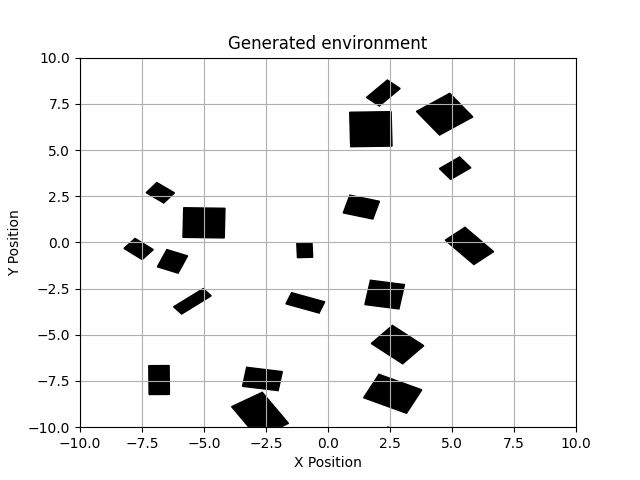
\includegraphics[scale=0.5]{asss3/images/pot4.png}
    \item \textbf{Number of obstacles}: 20
    \item \textbf{Start/goal configurations}: 
    \begin{enumerate}
        \item (1.5, 0.0) → (-5.0, 6.0)
        \item (4.0, 6.0) → (-7.0, -8.0)
        \item (-7.5, 4.0) → (-5.0, -8.0)
        \item (-1.0, 8.5) → (3.0, -4.0)
        \item (0.0, 8.5) → (8.5, -8.0)
    \end{enumerate}
    \item \textbf{Success rate}: 40\% (2/5) 
\textit{Failures}: For configurations 2, 3, and 4, the algorithm reached the maximum number of iterations. Start positions were likely too far from goal positions, necessitating more time and data to compute full paths.

    \item \textbf{Average duration of path search}: 0.0942 seconds
\end{itemize}

\subsubsection{Trial 5}

\begin{itemize}
    \item \textbf{Environment:}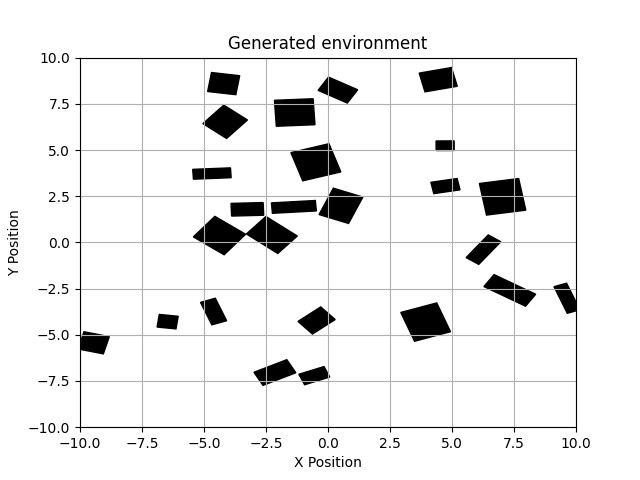
\includegraphics[scale=0.5]{asss3/images/pot5.png}
    \item \textbf{Number of obstacles}: 25
    \item \textbf{Start/goal configurations}: 
    \begin{enumerate}
        \item (1.5, 0.0) → (-5.0, 6.0)
        \item (2.5, 2.5) → (-2.5, -5.0)
        \item (-7.5, 4.0) → (-5.0, -8.0)
        \item (-1.0, 8.5) → (3.0, -4.0)
        \item (1.0, 0.5) → (-7.5, -8.0)
    \end{enumerate}
    \item \textbf{Success rate}: 40\% (2/5) 
\textit{Failures}: For configurations 2, 3, and 4, the algorithm reached the maximum number of iterations. Start positions were likely too far from goal positions, necessitating more time and data to compute full paths.

    \item \textbf{Average duration of path search}: 0.003325 seconds
\end{itemize}


\subsection*{2 Gtsam: Factor Graphs (Testing Report)}
Each trial was run with the following command:
python fg\_polynomial —initial 1 2 3 4

\subsubsection{Trial 1}
\begin{itemize}
    \item \textbf{Plot Visual:}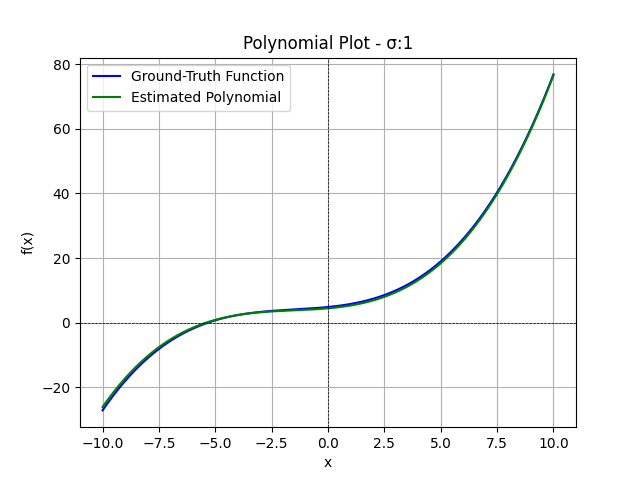
\includegraphics[scale=0.5]{asss3/images/poly1.png}
    \item \textbf{Ground Truth Polynomial}: $f(x)=0.045x^3+0.2x^2+0.7x+4.86$
    \item \textbf{Noise Level}: $σ=1$
    \item \textbf{Estimated Polynomial}: $f(x)=0.045086x^3+0.207x^2+0.623x+4.45$
\end{itemize}

\subsubsection{Trial 2}
\begin{itemize}
    \item \textbf{Plot Visual:}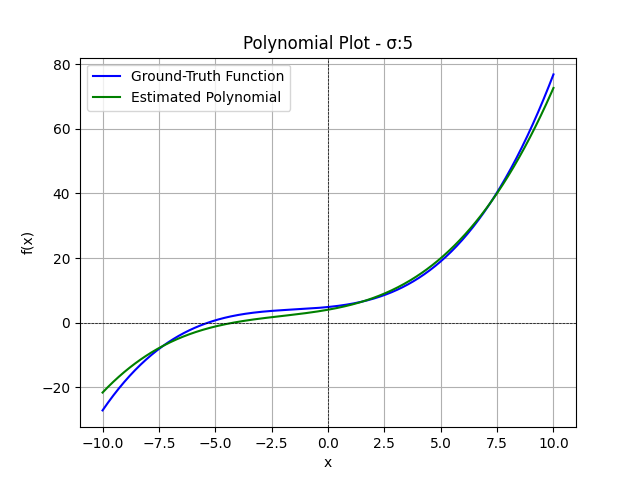
\includegraphics[scale=0.5]{asss3/images/poly2.png}
    \item \textbf{Ground Truth Polynomial}: $f(x)=0.045x^3+0.2x^2+0.7x+4.86$
    \item \textbf{Noise Level}: $σ=5$
    \item \textbf{Estimated Polynomial}: $f(x)=0.0346x^3+0.215x^2+1.24x+4.02$
\end{itemize}

\subsubsection{Trial 3}
\begin{itemize}
    \item \textbf{Plot Visual:}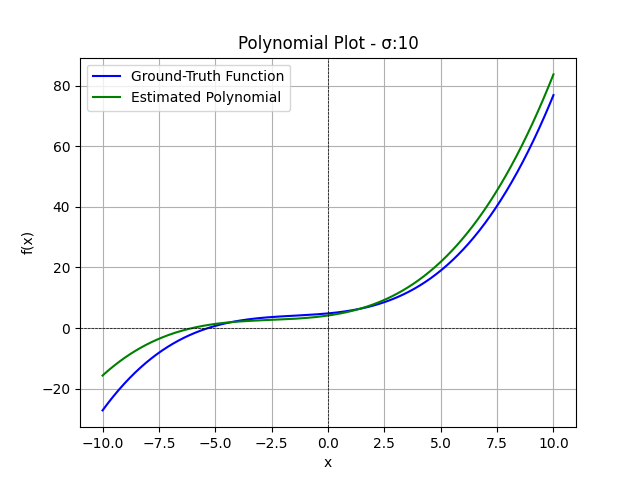
\includegraphics[scale=0.5]{asss3/images/poly3.png}
    \item \textbf{Ground Truth Polynomial}: $f(x)=0.045x^3+0.2x^2+0.7x+4.86$
    \item \textbf{Noise Level}: $σ=10$
    \item \textbf{Estimated Polynomial}: $f(x)=0.039x^3+0.298x^2+1.07x+4.16$
\end{itemize}


\subsection*{Trajectory Optimization via Factor Graphs}
\bfseries{3.1 Simple Trajectory}
\bfseries{\newline fg\_traj\_opt.py}
\begin{align*}
    \includegraphics[scale=0.2]{asss3/images/3.1 traj opt factor graph.PNG}
    \includegraphics[scale=0.2]{asss3/images/3.1 velocity over time.PNG}
\end{align*}
\begin{align*}
    \includegraphics[scale=0.2]{asss3/images/3.1 acceleration over time.PNG}
    \includegraphics[scale=0.2]{asss3/images/3.1 factor graph.PNG}
\end{align*}
\textbf{Factor Graph Diagram:}\texttt{ A diagram illustrating the factor graph with a few states (e.g., for \( T = 5 \)). Show the states \( q_t \), control inputs \( u_t \), and the factors connecting them (dynamics factors, control cost factors, acceleration cost factors, start and goal factors). }
\textbf{\newline Trajectory Optimization Graph: }\texttt{Please note that the blue line in the first image does not appear until you zoom in. This applies to all other graphs in this report as well.\newline}


\noindent\bfseries{3.2 Extra Constraints}
\bfseries{\newline fg\_traj\_opt\_2.py}
\begin{align*}
    \includegraphics[scale=0.2]{asss3/images/3.2 traj opt extra constraints.PNG}
    \includegraphics[scale=0.2]{asss3/images/3.2 factor graph.PNG}
\end{align*}
\begin{align*}
    \includegraphics[scale=0.2]{asss3/images/3.2 velocity.PNG}
    \includegraphics[scale=0.2]{asss3/images/3.2 acceleration.PNG}
\end{align*}
\textbf{Modified Factor Graph Diagram:} 
\texttt{A diagram of the factor graph highlighting the new intermediate state factors at \( T/3 \) and \( 2T/3 \).}

\textbf{\newline Trajectory Plot with Intermediate States:} 
\texttt{A plot showing the initial and optimized trajectories in the \( X \)-\( Y \) plane, including the intermediate states \( x_{\text{in}}^0 \) and \( x_{\text{in}}^1 \). Mark the key points (start, intermediate states, goal).}

\textbf{\newline Animation of the Trajectory (Not Shown):} 
\texttt{An animation showing the point moving along the optimized trajectory, visibly passing through the intermediate states.\newline}


\noindent\bfseries{3.3 2-Link Robot Arm}
\bfseries{\newline fg\_traj\_opt\_arm.py}
\begin{align*}
    \includegraphics[scale=0.2]{asss3/images/3.3 traj opt.PNG}
    \includegraphics[scale=0.2]{asss3/images/3.3 join angles.PNG}
\end{align*}
\begin{align*}
    \includegraphics[scale=0.2]{asss3/images/3.3 animation.PNG}
    \includegraphics[scale=0.2]{asss3/images/3.3 factor graph.PNG}
\end{align*}
\textbf{Factor Graph Diagram for Robot Arm:} 
\texttt{A diagram illustrating the factor graph for the 2-link robot arm, showing joint angles \( \theta_t \), control inputs \( u_t \), and the associated factors.}

\textbf{\newline Joint Angle Trajectory Plot:} 
\texttt{A plot of the initial and optimized trajectories in joint angle space (\( \theta_0 \) vs. \( \theta_1 \)).}

\textbf{\newline Animation of the Robot Arm:} 
\texttt{An animation showing the movement of the 2-link robot arm along the optimized trajectory.}

\subsection*{Trajectory Optimization in SE(2)}
\textbf{fg\_traj\_opt\_se2.py}
\begin{align*}
    \includegraphics[scale=0.2]{asss3/images/4 traj opt.PNG}
    \includegraphics[scale=0.2]{asss3/images/4 orientation.PNG}
\end{align*}
\begin{align*}
    \includegraphics[scale=0.2]{asss3/images/4 control inputs.PNG}
    \includegraphics[scale=0.2]{asss3/images/4 acceleration.PNG}
\end{align*}
\begin{align*}
    \includegraphics[scale=0.2]{asss3/images/4 traj animation.PNG}
    \includegraphics[scale=0.2]{asss3/images/4 factor graph.PNG}
\end{align*}
\textbf{Factor Graph Diagram in SE(2):} 
\texttt{A diagram of the factor graph representing poses \( q_t = (x_t, y_t, \theta_t) \), control inputs \( u_t \), and factors, including dynamics, control costs, acceleration costs, and constraints (start, goal, intermediate poses).}

\textbf{\newline Trajectory Plot in \( X \)-\( Y \) Plane:} 
\texttt{A plot showing the initial and optimized trajectories, including the start, goal, and intermediate poses. Mark key points for clarity.}

\textbf{\newline Orientation Over Time Plot:} 
\texttt{A plot of the robot's orientation \( \theta_t \) over time.}

\textbf{\newline Control Inputs and Acceleration Profiles:} 
\texttt{Plots of the control inputs (velocities) and accelerations over time.}

\textbf{\newline Animation of the Robot Trajectory:} 
\texttt{An animation showing the robot moving along the optimized trajectory in SE(2), passing through intermediate poses.}




\section*{Implementation Specifications}
\subsection*{potential.py}
\bfseries{Potential Functions}
\begin{itemize}
    \item \texttt{scene\_from\_file(filename)}
    \item \texttt{gradient\_repulsive\_potential(q, polygon)}
    \item \texttt{gradient\_potential(q, goal, obstacles)}
    \item \texttt{collisionCheckFreeBody(newPolygon, existingPolygon)}
    \item \texttt{pathCollisionCheck(p1, p2, polygon)}
    \item \texttt{line\_segment\_intersection(p1, p2, q1, q2)}
    \item \texttt{visualize\_robot\_path(q, robotCorners, obstacles, goal, path)}
\end{itemize}
\texttt{Description:}
\texttt{This code plans a robot's path in a 2D space using potential fields, where the robot is "pulled" toward a goal and "repelled" from obstacles. It loads an environment with obstacles from a file, calculates the attractive and repulsive forces, and updates the robot’s position using gradient descent. The robot stops when it reaches the goal or detects a collision-free path isn't possible.
In each step, the robot checks for collisions with obstacles using geometry and adjusts its movement by reducing the step size if necessary. The path is visualized in real-time, showing the robot navigating toward the goal while avoiding obstacles.}

%---------------------%

\subsection*{Gtsam: Factor Graphs}
\bfseries{fg\_polynomial.py}
\begin{itemize}
    \item \texttt{f(x, a=0.045, b=0.2, c=0.7, d=4.86)}
    \item \texttt{error\_func(y: np.ndarray, x: np.ndarray, this: gtsam.CustomFactor, v: gtsam.Values, H: List[np.ndarray])}
    \item \texttt{main()}
\end{itemize}
\texttt{Description:}\\
\texttt{The modified code extends the original linear regression implementation to fit a third-order polynomial by incorporating additional coefficients for higher-order terms (\(a, b, c, d\)) and their respective Jacobians. Key changes include updating the "true" function `f(x)` to a third-order polynomial \(f(x) = ax^3 + bx^2 + cx + d\), modifying `errorfunc` to handle four parameters and compute the partial derivatives (\(\frac{\partial \text{error}}{\partial a}, \frac{\partial \text{error}}{\partial b}, \frac{\partial \text{error}}{\partial c}, \frac{\partial \text{error}}{\partial d}\)) with respect to these parameters. In the main function, new keys (`ka`, `kb`, `kc`, `kd`) and initial guesses for these coefficients are defined, and the factor graph is built to model the polynomial relationship with added Gaussian noise. The implementation effectively uses GTSAM's `CustomFactor` and the Levenberg-Marquardt optimizer to estimate the coefficients, which are validated by comparing the noisy data to the estimated polynomial and the ground-truth function through visualization and printed results.}
%---------------------%

\subsection*{Trajectory Optimization via Factor Graphs}
\bfseries{3.1 Simple Trajectory}
\bfseries{\newline fg\_traj\_opt.py}
\begin{itemize}
    \item \texttt{dynamics\_factor(dt, t)}
    \item \texttt{start\_factor(start)}
    \item \texttt{goal\_factor(goal)}
    \item \texttt{control\_cost\_factor(t)}
    \item \texttt{acceleration\_cost\_factor(dt, t)}
    \item \texttt{visualize\_factor\_graph(T)}
\end{itemize}
\texttt{We implemented trajectory optimization for a point mass moving in 2D space using a factor graph. The variables are positions \( q_t \) and control inputs \( u_t \). The factors include dynamics factors enforcing \( q_{t+1} = q_t + u_t \Delta t \), start and goal factors enforcing the initial and final positions, and cost factors penalizing control efforts and accelerations to promote smoothness. The initial guess was a straight line from the start to the goal, with controls computed accordingly. \newline \newline}

\noindent\bfseries{3.2 Extra Constraints}
\bfseries{\newline fg\_traj\_opt\_2.py}
\begin{itemize}
    \item \texttt{dynamics\_factor(dt, t)}
    \item \texttt{start\_factor(start)}
    \item \texttt{goal\_factor(goal)}
    \item \texttt{intermediate\_factor(intermediate\_state, t)}
    \item \texttt{control\_cost\_factor(t)}
    \item \texttt{acceleration\_cost\_factor(dt, t)}
    \item \texttt{visualize\_factor\_graph(T)}
    \item \texttt{init()}
    \item \texttt{animate(i)}
\end{itemize}
\texttt{We extended the previous trajectory optimization by adding intermediate state constraints at times \( T/3 \) and \( 2T/3 \), ensuring the trajectory passes through specified points \( x_{\text{in}}^0 \) and \( x_{\text{in}}^1 \). New factors were added to the factor graph to enforce these constraints with large weights. The initial guess was constructed by piecewise linear interpolation through the start, intermediate states, and goal, providing a feasible starting point for optimization. \newline \newline}


\noindent\bfseries{2-Link Robot Arm}
\bfseries{\newline fg\_traj\_opt\_se2.py}
\begin{itemize}
    \item \texttt{wrap\_angles(angle)}
    \item \texttt{dynamics\_factor(dt, t)}
    \item \texttt{start\_factor(start)}
    \item \texttt{goal\_factor(goal)}
    \item \texttt{control\_cost\_factor(t)}
    \item \texttt{acceleration\_cost\_factor(dt, t)}
    \item \texttt{forward\_kinematics(theta)}
    \item \texttt{init()}
    \item \texttt{animate(i)}
    \item \texttt{visualize\_factor\_graph(T)}
\end{itemize}
\texttt{We implemented trajectory optimization for a 2-link robot arm, where the state is defined by joint angles \( q_t = (\theta_0, \theta_1) \). Factors in the graph include dynamics factors enforcing \( \theta_{t+1} = \theta_t + u_t \Delta t \), start and goal factors for initial and final joint angles, and cost factors penalizing control inputs and accelerations for smoothness. We handled angle wrapping manually to account for the periodic nature of joint angles. The initial guess was a linear interpolation between the start and goal angles.}

%---------------------%

\subsection*{Trajectory Optimization in SE(2) }
\bfseries{fg\_traj\_opt\_se2.py}
\begin{itemize}
    \item \texttt{wrap\_angle(angle)}
    \item \texttt{dynamics\_factor(dt, t)}
    \item \texttt{start\_factor(start)}
    \item \texttt{goal\_factor(goal)}
    \item \texttt{intermediate\_factor(intermediate\_pose, t)}
    \item \texttt{control\_cost\_factor(t)}
    \item \texttt{acceleration\_cost\_factor(dt, t)}
    \item \texttt{init()}
    \item \texttt{animate(i)}
    \item \texttt{visualize\_factor\_graph(T)}
\end{itemize}
\texttt{We extended trajectory optimization to \( SE(2) \) by optimizing over poses \( q_t = (x_t, y_t, \theta_t) \) and control inputs \( u_t \). The factor graph includes dynamics factors enforcing \( q_{t+1} = q_t + u_t \Delta t \) with angle wrapping for \( \theta_t \), start and goal factors, intermediate pose constraints, and cost factors penalizing control inputs and accelerations. The initial guess was generated by interpolating between waypoints (start, intermediate poses, goal) with proper angle wrapping to ensure continuity.}





\end{document}
